% Cascade P→PI position control (industry-standard servo architecture).
% Compile: pdflatex position-loop-cascade-p.tex && pdf2svg ...
\documentclass[tikz, margin=4mm]{standalone}
\usetikzlibrary{arrows.meta, positioning, calc}

\tikzset{
  block/.style = {draw, rectangle, rounded corners=2pt, align=center,
                  fill=blue!8, font=\small,
                  minimum height=1.0cm, minimum width=2.4cm},
  sum/.style   = {draw, circle, fill=blue!8, minimum size=7mm, inner sep=0pt},
  arr/.style   = {-{Latex[length=4pt, width=5pt]}, thick},
  lbl/.style   = {font=\footnotesize},
  node distance = 0.9cm and 1.8cm
}

\begin{document}
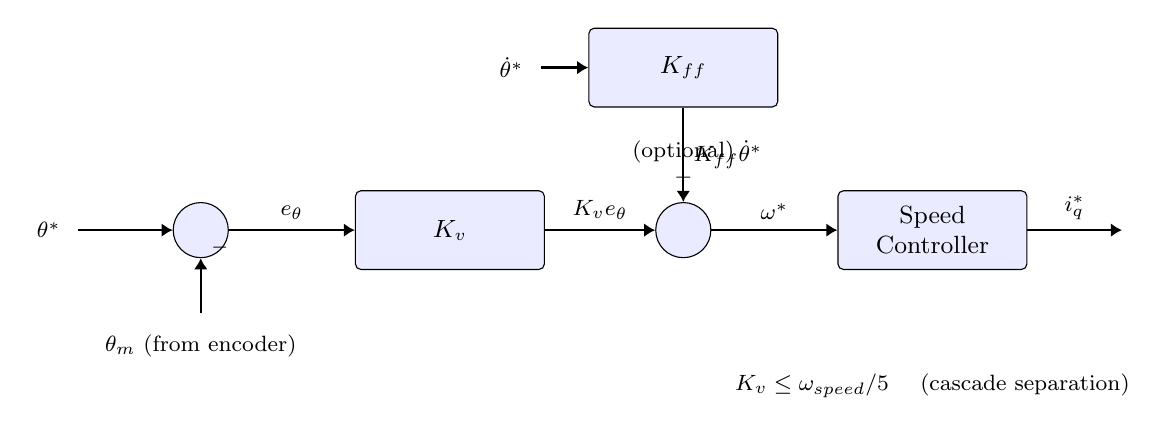
\begin{tikzpicture}

  % ── Position loop ─────────────────────────────────────────────────────────
  \node[sum]                           (Sth)    {};       % θ error
  \node[block, right=1.6cm of Sth]     (Kv)     {$K_v$};  % position gain
  \node[sum,   right=1.4cm of Kv]      (SFF)    {};       % velocity FF summing

  % ── Speed loop (inner) ────────────────────────────────────────────────────
  \node[block, right=1.6cm of SFF]     (Spd)    {Speed\\ Controller};

  % ── Velocity feedforward (optional) ───────────────────────────────────────
  \node[block, above=1.2cm of SFF]     (KFF)    {$K_{ff}$};

  % ── I/O ───────────────────────────────────────────────────────────────────
  \coordinate (ThRef)  at ($(Sth.west)+(-1.2,0)$);
  \coordinate (ThDotIn) at ($(KFF.west)+(-0.6,0)$);
  \coordinate (IqOut)  at ($(Spd.east)+(1.2,0)$);
  \coordinate (ThFb)   at ($(Sth.south)+(0,-0.7)$);

  % ── Connections ───────────────────────────────────────────────────────────

  % Position reference
  \node[lbl, left=0.1cm of ThRef] {$\theta^*$};
  \draw[arr] (ThRef) -- (Sth);

  % Position error → Kv → ω* summing
  \draw[arr] (Sth) -- node[lbl,above]{$e_\theta$}  (Kv);
  \draw[arr] (Kv)  -- node[lbl,above]{$K_v e_\theta$} (SFF);

  % Velocity feedforward path
  \node[lbl, left=0.1cm of ThDotIn] {$\dot{\theta}^*$};
  \draw[arr] (ThDotIn) -- (KFF);
  \draw[arr] (KFF) -- node[lbl,right]{$K_{ff}\dot{\theta}^*$} (SFF);

  % ω* to speed controller
  \draw[arr] (SFF)  -- node[lbl,above]{$\omega^*$} (Spd);
  \draw[arr] (Spd.east) -- node[lbl,above]{$i_q^*$} (IqOut);

  % Position feedback (negative)
  \node[lbl, below=0.15cm of ThFb] {$\theta_m$ (from encoder)};
  \draw[arr] (ThFb) -- (ThFb -| Sth) -- (Sth)
             node[below right, font=\scriptsize]{$-$};

  % Constraint note
  \node[lbl, below=1.2cm of Spd] {$K_v \leq \omega_{speed}/5$ \quad (cascade separation)};
  \node[lbl, below=0.3cm of KFF] {(optional)};

  % + sign on velocity FF summing junction
  \node[font=\scriptsize, above=0.1cm of SFF] {$+$};

\end{tikzpicture}
\end{document}
